 \documentclass{report}
 
\usepackage[utf8]{inputenc} 
\usepackage[T1]{fontenc}      
\usepackage[top=2.0cm, bottom=3cm, left=3.0cm, right=3.0cm]{geometry}
\usepackage{graphicx}
\usepackage{wrapfig}
\usepackage{amsmath,esint }
\usepackage{amssymb}
\usepackage{esvect}

\graphicspath{{figures/}{../figures}}

\newcommand*\dif{\mathop{}\!\mathrm{d}}
\newcommand*\diver{\mathop{}\!\mathrm{div}}
\newcommand*\grad{\mathop{}\!\mathrm{grad}}

\begin{document}

\section*{Approche ontologique du champ magnétique}

\subsubsection*{Approche en mécanique classique}

\begin{itemize}
	\item[$\clubsuit$] Dans une volume $a\Sigma$, on a une charge $+e$ et une charge $-e$, comme celle-ci sont réparties uniformément. Les densités de charges sont donc respectivement $\rho_+=e/(a\Sigma)$ et $\rho_-=-e/(a\Sigma)$.
	\item[$\clubsuit$] Par définition, $\vec{j}=\rho\vec{v}$. Comme seuls les électrons ont une vitesse non nulle, $\vec{j}=\rho_-\vec{v'}=ev'/(a\Sigma)\vec{e}_x$. Et donc $I=\oiint_\Sigma\dif\vec{S}\vec{j}=ev'/a$.
	\item[$\clubsuit$] $\rho_{tot}=\rho_++\rho_-=0$ donc $\vec{E}=0$.
	\item[$\clubsuit$] Avec le théorème d'Ampère appliqué uniquement en dehors du fil, on trouve :
	\begin{align*}
		\vec{B}=\frac{\mu_0I}{2\pi r}\vec{e_\theta}
	\end{align*}
	(résultat classique d'un fil parcouru par un courant $I$)
	La force qui s'exerce sur la charge $q$ est donc :
	\begin{align*}
		\vec{F}=-\frac{qv\mu_0I}{2\pi r}\vec{e_r}
	\end{align*}
\end{itemize}

\subsubsection*{Approche en mécanique relativiste}

	\begin{itemize}
	
		\item[$\clubsuit$] Ainsi, en se déplaçant à la vitesse $\vec{v}$, la charge $+q$ voit dans son référentiel la distance entre atomes réduite d'un facteur $\gamma_{+}=1/\sqrt{1-v^{2}/c^{2}}$ et la distance entre électrons de conduction d'un facteur $\gamma_{-}=1/\sqrt{1-(v-v')^{2}/c^{2}}$. 
		On trouve donc que :
		\begin{align*}
			\rho_+=\frac{e}{a\Sigma}\sqrt{1-v^{2}/c^{2}}
		\end{align*}
		\begin{align*}
			\rho_-=\frac{e}{a\Sigma}\sqrt{1-(v+v')^{2}/c^{2}}
		\end{align*}		
		Attention, l'hypothèse que la vitesse relative des électrons par rapport à la charge $q$ est $v'+v$ est une approximation. En mécanique relativiste, la vitesse relative serait :
		\begin{equation}
			v_{e_-/q}=\frac{v'-v}{1-\frac{vv'}{c^2}}
		\end{equation}
		
	\item[$\clubsuit$] On trouve facilement avec le théorème de Gauss que :
	\begin{align*}
		\vec{E}=\frac{\Sigma(\rho_++\rho_-)}{2\pi r\varepsilon_0}
	\end{align*}
	
	 En développant à l'ordre 2, on trouve :
	\begin{align*}
		\rho_++\rho_-\approx -\frac{e}{a\Sigma}\frac{vv'}{c^2}
	\end{align*}
	On trouve alors que :
	\begin{align*}
		\vec{E}=-\frac{e vv'}{2\pi r a\varepsilon_0 c^2}\vec{e_r}=-\frac{I\mu_0 v}{2\pi r}\vec{e_r}
	\end{align*}
	
	\item[$\clubsuit$]
	La force de Lorentz associée est donc :
	\begin{align*}
		\vec{F}=-\frac{qe vv'}{2\pi r a\varepsilon_0 c^2}\vec{e_r}=-\frac{qI\mu_0 v}{2\pi r}\vec{e_r}
	\end{align*}
	
	Cette expression est identique à celle trouvée par le calcul du champ magnétique en mécanique classique. Le champ magnétique est-il est une approximation à l'ordre 2 de la force de Coulomb ? 
	\end{itemize}

\section*{Corrosion en phase acqueuse}

\subsubsection*{Corrosion uniforme du zinc en milieu acide}

\begin{itemize}
	
	\item[$\clubsuit$] Le potentiel de Nernst est $E_n=E^0=-0.76$V comme la concentration de zinc est de 1mol/L.
	
	\begin{figure}[h!]
	\centering
			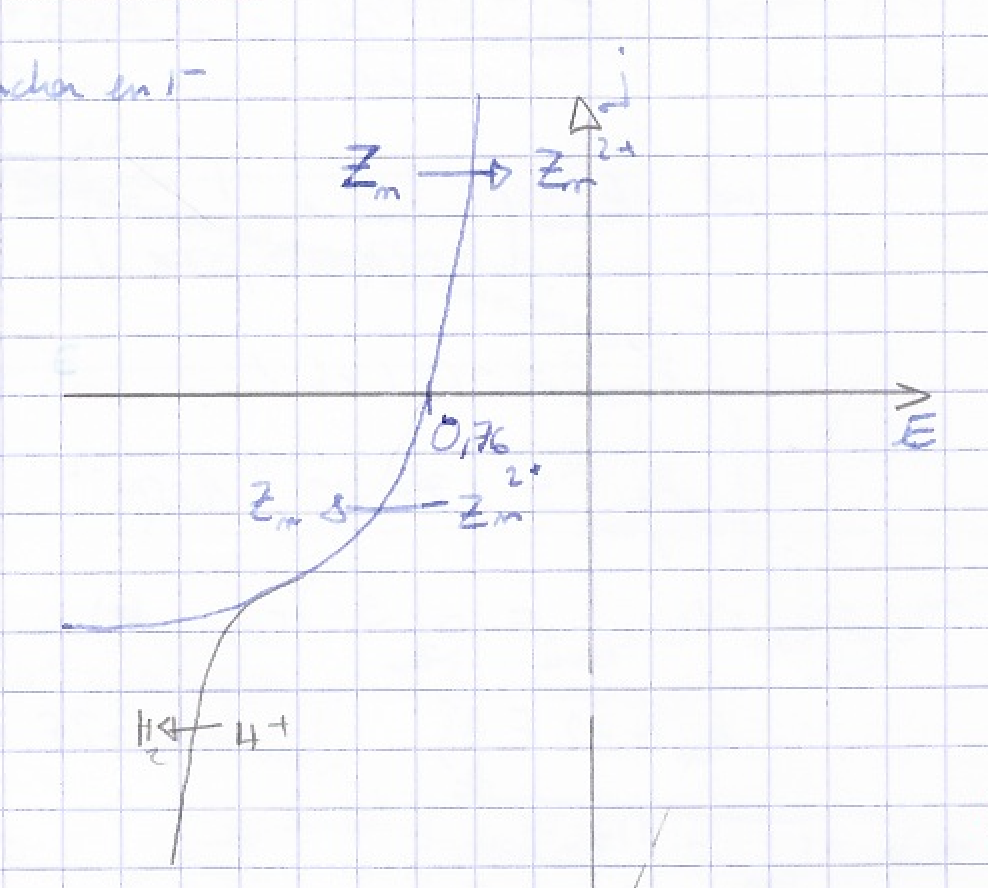
\includegraphics[scale=0.25]{pot_zn.png}
	\end{figure}	
	
	\item[$\clubsuit$] Oui, le type de métal peut modifier la surtension (minimale pour le platine) mais aussi l'état de surface : plus la surface de réaction est grande, moins celle-ci sera limitée par la diffusion des ions $H^+$. Par défaut, on suppose que le pH est acide, à 0, comme suggéré dans l'énoncé. 
	
	\begin{figure}[h!]
	\centering
			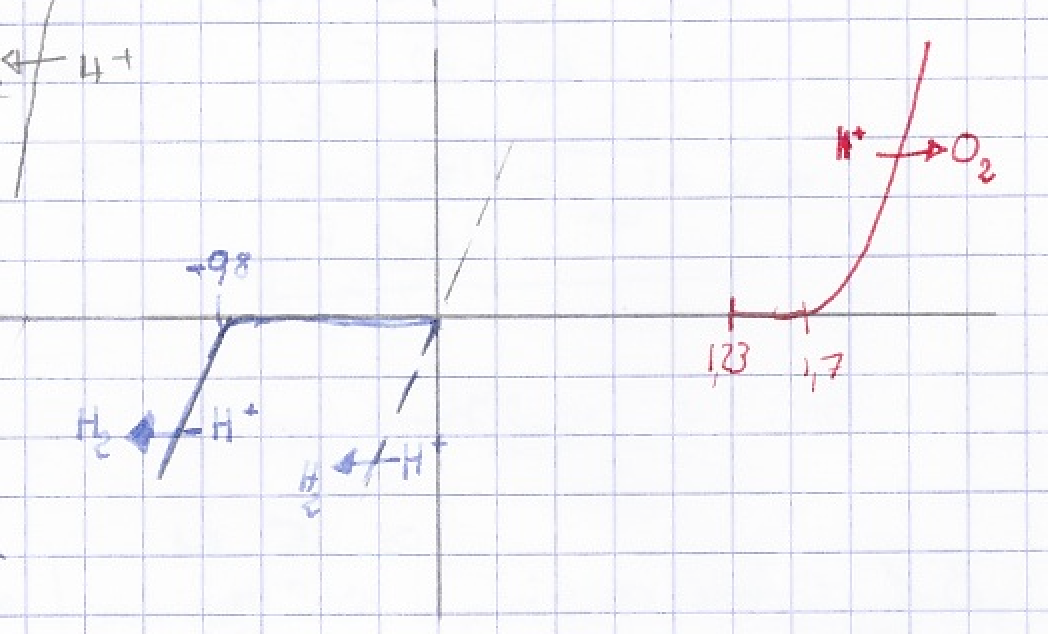
\includegraphics[scale=0.25]{pot_h.png}
	\end{figure}	
	
	\item[$\clubsuit$] $Zn+2H^+\longrightarrow Zn^{2+}+H_2$. On rappelle pour que pour voir ce qu'il se passe en oxydation, la première réaction qui se fait est celle de plus bas potentiel. En réduction, la première réaction est celle de plus haut potentiel. Cette réaction est thermodynamiquement possible car $E^0_{Zn/Zn^{2+}}<E^0_{H^+/H_2}$
	
	\item[$\clubsuit$] Par conservation du courant, $i_a+i_c=0$. comme les surfaces des deux électrodes sont les mêmes, on trouve $j_a+j_c=0$.
	
\end{itemize}

\section*{Exercice 3}

\begin{itemize}
	
	\item[$\spadesuit$] Entre $t$ et $t+dt$, le nombre d'électrons ayant subi une collision est $N(t)\frac{dt}{\tau}$ : en effet, à $t$ il reste $N(t)$ électrons n'ayant pas collisioné et parmi eux, une proportion $\frac{dt}{\tau}$ va subit une collision durant $dt$. A noter que cela est valable dans le cadre de la loi des grand nombre, qui est largement validée ici au vu des quantité d'électrons dans un métal.
	
	On en déduit alors que le nombre d'électrons n'ayant pas collisioné à $t+dt$ est :
	\begin{align*}
		N(t+dt) = N(t) - N(t)\frac{dt}{\tau}
	\end{align*}
	On tombe sur l'équation différentielle classique de la désintgration radioactive, donnée par $\dot{N}(t)=-\frac{1}{\tau}N(t)$.En intégrant, on trouve la relation voulue.
	
	\item[$\spadesuit$] La probabilité pour un électron de ne pas subir de collision jusqu'à l'instant $t$ correspond au nombre total d'électrons n'yant pas subi de collision sur le nombre total d'électrons, soit $N(t)/N_0=\exp(-t/\tau)$. 
	
	La probabilité $dp$ pour un électron de subir une collision entre $t$ et $t+dt$ correspond à la \textit{probabilité de ne pas avoir subi de collision jusqu'à} $t$ ET à la \textit{probabilité de subir une collision entre $t$ et $t+dt$}, soit le produit de probabilité :
	\begin{align*}
		dp = \exp(-t/\tau)\cdot\frac{dt}{\tau}
	\end{align*}
La valeur moyenne du temps de collision correspond à la somme des temps $t$ durant laquelle il y a eu collision multiplié par la probabilité de collision entre $t$ et $t+dt$ :
	\begin{align*}
		\bar{t}=\int_0^{\infty}tdp=\int_0^{\infty} t\exp(-t/\tau)\cdot\frac{dt}{\tau}=\tau
	\end{align*}
	
	\item[$\spadesuit$] Soit $N_0$ le nombre total d'électrons. Entre $t$ et $t+dt$, il y a eu $dtN_0/\tau$ qui ont subi une collision. La quantité de mouvement de tous ces électrons est donc perdue. D'autre part, entre $t$ et $t+dt$ chaque électron est soumis à la force $\vec{F}(t)$, faisant changer la quantité de mouvement totale de $N_0F(t)dt$. Finalement, il vient :
	\begin{equation}
		\vec{P}(t+dt)=\vec{P}(t)-\frac{dt}{\tau}\vec{P}(t)+N_0\vec{F}dt
	\end{equation}
	
	\item[$\spadesuit$] On en déduit la vitesse moyenne d'un électron, définie par $\vec{v}(t)=\vec{P}/(mN_0)$ :
	\begin{align*}
		\frac{d\vec{v}}{dt}=\frac{\vec{v}}{\gamma}+\vec{F}(t)
	\end{align*}
	où $\gamma=m/\tau$.
	
	\item[$\spadesuit$] La force subie par les électrons est la force de Lorentz : $\vec{F}=-eE_0\exp(-i\omega t)$. L'équation précédente devient :
	\begin{align*}
		-i\omega\vec{v}=-\frac{e}{m}\vec{E_0}-\frac{\vec{v}}{\tau}
	\end{align*}
	On en déduit :
	\begin{align*}
		\vec{v}=\frac{e\tau}{m}\frac{E_0}{i\omega\tau-1}
	\end{align*}
	En introduisant la conductivité $\gamma$, $\vec{j}=\gamma \vec{E}$, où $\vec{j}=-ne\vec{v}$, on trouve :
	\begin{align*}
		\gamma(\omega)=\frac{ne^2\tau}{m}\frac{1}{1-i\omega\tau}
	\end{align*}
	
	\item[$\spadesuit$] Dans un métal, qui est un réseau cristallin, il y a typiquement un électron tous les Angstrom, soit tous les $10^{-10}$m. On obtient des densités typiques de $10^{30}$ atomes par m$^3$.
	
	\item[$\spadesuit$] La résistivité statique correspond à une fréquence qui tend vers 0, cad :
	\begin{align*}
		\rho = \frac{1}{\gamma}=\frac{m}{ne^2\tau}
	\end{align*}
	On trouve donc $\tau\simeq10^{-14}$s.
	
\end{itemize}

\newpage

\section*{Conduction électrique dans un semiconducteur bidimensionnel}

\begin{itemize}

	\item[$\bowtie$] $\vec{j_s}=-en_s\vec{v}$ et $\vec{j_s}=I/W$.

	\item[$\bowtie$] Entre $t$ et $t+dt$, les électrons ont acquis une quantité de mouvement $-eN_0\vec{E}dt$, mais en ont perdu par collision $-P(t)dp=-P(t)\times dt/\tau$ (comme une fraction $dt/\tau$ d'électrons ont perdu \textbf{en moyenne} leur quantité de mouvement). On a donc :
	\begin{align*}
		P(t+dt) = P(t)-eN_0\vec{E}dt-P(t)\frac{dt}{\tau}
	\end{align*}
	En régime permanent, $P(t+dt) = P(t)$, donc :
	\begin{align*}
		\vec{P}=-eN_0\tau\vec{E}
	\end{align*}
	Et alors :
	\begin{align*}
		\vec{v}=-\frac{e\tau}{m}\vec{E}
	\end{align*}
	
	\item[$\bowtie$] Le courant surfacique est donc :
	\begin{align*}
		\vec{j_s}=\frac{e^2\tau n_s}{m}\vec{E}
	\end{align*}
	
	Et comme $V_1-V_2 = int_1^2\vec{dl}\cdot \vec{E}=E\times L$ et que $I=j_S\times W$, on obtient :
	\begin{align*}
		V_1-V_2 = I\times\frac{m}{e^2\tau n_s}\frac{L}{W}
	\end{align*}
	Donc $R_\boxdot = \frac{m}{e^2\tau n_s}\frac{L}{W}$
	
	\item[$\bowtie$] $R_\boxdot$ ne dépend que du rapport d'aspect du conducteur (qui est rectangulaire) : dans le cas $W=L$, la résistance ne dépend plus des dimensions du conducteur. Pour connaitre la resistance d'un tel conducteur, il suffit de "compter" les carrés composant le conducteur (et faire les lois d'addition de résistance en série et en parallèle) pour en déduire la résistance totale du conducteur.
	
	\item[$\bowtie$] On note $x$ la dimsension le long du conducteur (selon $l$) et on décompose le conducteur en 3 parties : la première partie du sablier, le carré central et la seconde partie en sablier, notées 1, 2 et 3.
	
	Dans la partie $1$, on a $j_s=I/(w-ax)$, avec $a=\frac{l}{W-d}$. Comme on a toujours $\vec{j_s}=\frac{e^2\tau n_s}{m}\vec{E}$, on obtient :
	\begin{align*}
		\Delta V_1=\frac{m}{e^2\tau n_s}\int_{x=0}^{x=l}dxj_s(x)=\frac{m}{e^2\tau n_s}\times\frac{I}{a}\ln\left(\frac{w}{d} \right) 
	\end{align*}
	où $\Delta V_1 = V_1-V(x=l)$ est la chute de tension dans la partie 1. On a $\Delta V_1+\Delta V_2+\Delta V_3=V_1-V_2 = E\times (2l+d) $.
	
	Finalement, on obtient :
	\begin{align*}
		R_1=\frac{m}{e^2\tau n_sa}\ln\left(\frac{w}{d} \right) =\frac{R_\boxdot}{a}\ln\left(\frac{w}{d} \right)
	\end{align*}
	
	Comme la résistance centrale est une résistance "carrée", on a $R_2=R_\boxdot$. Enfin, par symétrie, on a $R_1=R_3$. Donc :
	\begin{align*}
		R = R_1+R_2+R_3 = R_\boxdot\left(\frac{2}{a}\ln\left(\frac{w}{d} \right)+1 \right) 
	\end{align*}
	
	
	\item[$\bowtie$] $p_s=\vec{j_s}\cdot\vec{E}=\frac{I}{l(x)}\times\frac{V_1-V_2}{2l+d}$, où $l(x)$ est la largeur du conducteur en $x$. 
	
	La puissance totale est donc :
	\begin{align*}
	P_J = \iint dx dy\times p_s = \int_{0}^{2l+d} dx l(x)\times\frac{I}{l(x)}\times\frac{V_1-V_2}{2l+d} = (V_1-V_2)\times I= RI^2
	\end{align*}

\end{itemize}

\section*{Exercice 4}

\begin{itemize}

	\item[$\heartsuit$] Résistance classique d'un cylindre : $R=L/(\gamma\pi a^2)$.
	
	\item[$\heartsuit$] Isolons le câble arrivant en $A$. Par symétrie, le courant $I$ partira dans tous les directions. La densité de courant va s'écrire en un point $M$ :
	\begin{align*}
		\vec{j_A}=\frac{I}{2\pi e }\frac{\vec{AM}}{\|\vec{AM} \|^2}
	\end{align*}
	C'est une décroissance typique en $1/r$, où $r=AM$.
	On effectue le même raisonnement pour la source de courant en $B$, mais où la source de courant est $-I$. Par superposition, la densité de courant totale est alors :
	\begin{align*}
		\vec{j}=\frac{I}{2\pi e }\left[ \frac{\vec{AM}}{\|\vec{AM} \|^2} - \frac{\vec{BM}}{\|\vec{BM} \|^2}\right] 
	\end{align*}
	
	\item[$\heartsuit$] En intégrant la relation $\vec{j}=\gamma\vec{E}$ le long du chemin $AB$, dont la coordonnée sera donnée par $x$, en faisant varier $x$ de $a$ à $d-a$ (pour éviter une divergence de la densité de courant) :
	\begin{align*}
		\int_a^{d-a}dx j(x)=\frac{I}{2\pi e}\int_a^{d-a}dx\left(\frac{1}{x}+\frac{1}{d-x} \right) =\gamma\int_a^{d-a}dxE=-\gamma\int_a^{d-a}dx\frac{dV}{dx}
	\end{align*}
	
	\textit{Remarque} : Lorsque $M$ est strictement contenu sur le segment $AB$, on a : $\vec{BM} = -\|BM\|\vec{e}_x=-(d-a)\vec{e}_x$ où $\vec{e}_x$ est le vecteur normé orientant ce segment. 
	
	On trouve alors :
	\begin{align*}
		\Delta V = \frac{I}{\pi e\gamma}\log\left(\frac{d-a}{a} \right) 
	\end{align*}

	\item[$\heartsuit$] En se plaçant en coordonnées sphériques, on a :
	\begin{align*}
		\vec{j}=\frac{I}{2\pi}\left[ \frac{\vec{e_r}}{\|\vec{AM} \|^2} - \frac{\vec{e_r}}{\|\vec{BM} \|^2}\right] 
	\end{align*}
	Attention, il y a un facteur 2 par rapport à la surface d'une sphère car il s'agit de demi-sphères.
		On trouve alors :
	\begin{align*}
		\Delta V = \frac{I}{\pi \gamma}\frac{d}{a(d-a)}
	\end{align*}
	
\end{itemize}

\section*{Exercice 5}

\begin{itemize}

	\item[$\diamondsuit$] Les lignes de champs sont radiales cad $\vec{j}=j(r)\vec{e_r}$. On a donc :
\begin{align*}
	\vec{j}(r)=\frac{I}{2\pi r^2}\vec{e_r}
\end{align*}
On en déduit :
\begin{align*}
	\dif V=-E(r)dr=\frac{-I}{2\pi r^2\gamma}dr
\end{align*}
Par intégration, on trouve :
\begin{align*}
	V(r)=\frac{I}{2\pi r\gamma}
\end{align*}

	\item[$\diamondsuit$] Le potentiel de l'hémisphère est donc simplement :
\begin{align*}
	U=\frac{I}{2\pi a\gamma}
\end{align*}
La résistance est donc tout simplement $R=\frac{1}{2\pi a \gamma}$. On trouve qu'elle ne dépasse pas 30$\Omega$ si $a>53$cm.

	\item[$\diamondsuit$] La tension de pas vaut, si $d=1$m :
	\begin{align*}
		V_p(r)=V(r)-V(r+d)=\frac{I}{2\pi \gamma r(r+d)}
	\end{align*}
On trouve que $V_p(10m)=7,2kV$ et  $V_p(100m)=79V$

	\item[$\diamondsuit$] Le courant qui traverse la personne est $i=V_p/R$. On trouve i(10)=2,9A et i(100)=32mA.
\end{itemize}

\section*{Câble coaxial}

\begin{itemize}

	\item[$\heartsuit$] Le courant circulant dans l'âme est $I=2\pi a j_{s,a}$. De même, la charge totale est $Q=2\pi a l \sigma_a$. On a forcément $I=2\pi b j_{s,b}$. De même, la charge totale est $Q=2\pi b l \sigma_b$ par conservation de la charge et du courant. 
	
	\item[$\heartsuit$] Les symétries et les invariances donnent $\vec{E}=E(r)\vec{e_r}$. Avec le théorème de Gauss appliqué sur un cylindre de rayon $r$, on obtient :
	\begin{align*}
	\left\lbrace
	\begin{array}{ccc}
	r<a & : & \vec{E}=\vec{0} \\
	a<r<b & : & \vec{E} = \frac{\sigma_a a}{\varepsilon_0 r}\vec{e_r} \\
	r>b & : & \vec{E}=\vec{0}
	\end{array}\right.
\end{align*}

	\item[$\heartsuit$] On en déduit le potentiel entre les deux conducteurs :
	\begin{align*}
		V=\frac{\sigma_aa}{\varepsilon_0}\ln\left(\frac{b}{a} \right) =\frac{Q}{2\pi l\varepsilon_0}\ln\left(\frac{b}{a} \right)
	\end{align*}
La capacité par unité de longueur est donc :
\begin{align*}
	c = \frac{2\pi\varepsilon_0}{\ln\left(\frac{b}{a} \right)}
\end{align*}

	\item[$\heartsuit$] Les symétries et les invariances donnent $\vec{B}=B(r)\vec{e_\theta}$. Avec le théorème de d'Ampère appliqué sur un cercle de rayon $r$, on obtient :
	\begin{align*}
	\left\lbrace
	\begin{array}{ccc}
	r<a & : & \vec{B}=\vec{0} \\
	a<r<b & : & \vec{B} = \frac{\mu_0j_{s,a} a}{r}\vec{e_\theta} \\
	r>b & : & \vec{B}=\vec{0}
	\end{array}\right.
\end{align*}

	\item[$\heartsuit$] Le flux du champ $\vec{B}$ se calcule sur la surface rectangulaire comprises entre $a$ et $b$, de longueur $l$ avec $\vec{e_\theta}$ comme vecteur normal. On trouve alors :
	\begin{align*}
		\Phi_B=\frac{L\mu_0I}{2\pi}\ln\left(\frac{b}{a} \right)
	\end{align*}
	On a donc :
	\begin{align*}
		l=\frac{\mu_0}{2\pi}\ln\left(\frac{b}{a} \right)
	\end{align*}

	\item[$\heartsuit$] On trouve que $l\times c=\varepsilon_0\mu_0=\frac{1}{c^2}$. Cela correspond à l'inverse du carré de la vitesse de la lumière, qui est la vitesse de propagation dans le câble coaxial.
	
\end{itemize}

\section*{Étude d'un colloïde}

\begin{itemize}

	\item[$\heartsuit$] Classique, champ électrique généré par le potentiel d'une charge $Q$ :
	\begin{align*}
		\vec{E}=\frac{Q}{4\pi\varepsilon_0 r^2}\vec{e_r}
	\end{align*}
 Et, en prenant le potentiel nul à l'infini :
	\begin{align*}
		V=\frac{Q}{4\pi\varepsilon_0 r}
	\end{align*}
Si $Q>0$, on aura les ions négatifs qui vont venir s'agglutiner autour de la charge $Q$, alors que les ions positifs seront plus repoussés plus loin. Le problème est que cette répartition d'ions n'est pas "stable" car il faut tenir compte du potentiel des ions lors de la nouvelle répartition. 	
	
	\item[$\heartsuit$] Le milieu est composé de cations et d'anions à la même densité :
	\begin{align*}
		\rho=eN_+-eN_-=-2eN_0\sinh\left( \frac{eV}{k_BT}\right) 
	\end{align*}
Lorsque $eV\ll k_BT$, on a alors : 
\begin{align*}
	\rho\simeq -2N_0\frac{eV}{k_BT}
\end{align*}

	\item[$\heartsuit$] Avec les rotations et les symétries, on montre facilement que $\vec{E}=E(r)\vec{e_r}$. On applique le théorème de Gauss sur un volume compris entre $r$ et $r+dr$ :
	\begin{align*}
		-4\pi r^2E(r)-4\pi(r+\dif r)^2E(r+\dif r)=\frac{4\pi r^2\dif r\rho}{\varepsilon}
	\end{align*}
	On trouve donc :
	\begin{align*}
		\frac{1}{r^2}\frac{\dif}{\dif r}\left( r^2\frac{\dif V}{\dif r}\right) +\frac{\rho}{\epsilon}=0
	\end{align*}
	Cette éuation correspond à l'équation de Maxwell-Gauss : $\diver\vec{E}=\frac{\rho}{\varepsilon}$ (qui correspond à l'équation de Poisson avec le potentiel).

	\item[$\heartsuit$] On remplace $\rho$ par l'expression trouvée plus haut. On obtient : 
	\begin{align*}
		\frac{\dif^2U}{\dif r^2}-\frac{2N_0e^2}{k_BT\varepsilon}U=0
	\end{align*}
	
	On pose $\lambda^2 = \frac{k_BT\varepsilon}{2N_0e^2}$. C'est une longueur caractéristique de la décroissance du potentiel. Dans de l'eau pure, le pH est égal à 7 donc $N_0=10^{-7}$mol/L$=10^{19}$part.m$^{-3}$, soit $\lambda=1\mu$m.
	
	En résolvant l'équation, on trouve $U(r)=A\exp\left(-r/\lambda \right) +B\exp\left(r/\lambda\right)$. La condition aux limites $V(r\longrightarrow\infty)\longrightarrow0$ impose $B=0$. On a alors :
	\begin{align*}
		V(r)=\frac{A}{r}\exp\left(-\frac{r}{\lambda} \right) 
	\end{align*}
	
	\item[$\heartsuit$] L'expression du champ est :
	\begin{align*}
		\vec{E}=-\frac{\dif V}{\dif r}\vec{e_r}=A\frac{\exp(-r/\lambda)}{r^2}\left(1+\frac{r}{\lambda}\right)\vec{e_r}
	\end{align*}
	S'il n'y avait pas d'ions, on devrait retrouver l'expression du champ d'une particule ponctuelle de charge $Q$. Or l'absence d'ions correspond à $\lambda=\infty$, c'est-à-dire qu'il n'y a plus d'écrantage. On doit nécessairement retrouver $\vec{E}=\frac{Q}{4\pi\epsilon r^2}\vec{e_r}$.
	
	D'autre part, pour $r=r_0$, l'expression du champ \textit{avec} ou \textit{sans} ions autour est la même (car on est collé à la surface de la particule). Donc :
	\begin{align*}
		\frac{Q}{4\pi\epsilon r^2}=A\frac{\exp(-r_0/\lambda)}{r^2}\left(1+\frac{r_0}{\lambda}\right)
	\end{align*}
	
	On a alors :
	\begin{align*}
		V(r)=\frac{Q}{4\pi\epsilon r^2}\frac{1}{1+\frac{r_0}{\lambda}}\exp\left(-\frac{r-r_0}{\lambda} \right) 
	\end{align*}
	Le potentiel décroit très rapidement avec la distance (beaucoup plus rapidement que si la charge était seule).
	
	\item[$\heartsuit$] La densité de charge est proportionnelle à l'opposé du potentiel :
	\begin{align*}
		\rho(r)=-\frac{2N_0eQ}{4\pi k_BT\epsilon r^2}\frac{1}{1+\frac{r_0}{\lambda}}\exp\left(-\frac{r-r_0}{\lambda} \right) 
	\end{align*}	
	Cette densité de charge est opposée à la charge $Q$ : les ions de signe opposés s'agglutinent bien autour de la charge $Q$. D'autre part, le potentiel décroit rapidement : celui créé par la charge $Q$ disparait rapidement, à cause de l'aglutinement des ions autour. Ils écrantent sa charge.
	
	\item[$\heartsuit$] Dans le cas où $N_0=10^{-7}$mol/L, la concentration en ions est 100 fois supérieure à celle de l'eau pure et $\lambda$ est donc inférieur d'un facteur 10. Le champ électrique chutant très rapidement avec la distance, plus on rajoute d'ions, plus l'effet d'une particule à l'autre sera faible, et moins les particules de colloïde se repousseront naturellement. Elles auront tendance à tomber au fond de la solution.
	
\end{itemize}

\section*{Condensateur Terre-ionosphère}

\begin{itemize}

	\item[$\clubsuit$] Les symétries et les invariances donnent $\vec{E}=E(r)\vec{e_r}$. Avec le théorème de Gauss appliqué sur une sphère de rayon $r$, on obtient :
	\begin{align*}
	\left\lbrace
	\begin{array}{ccc}
	r<R & : & \vec{E}=\vec{0} \\
	R<r<R+z_0 & : & \vec{E} = -\frac{Q}{4\pi\varepsilon_0 r^2}\vec{e_r} \\
	r>R+z_0 & : & \vec{E}=\vec{0}
	\end{array}\right.
\end{align*}

	\item[$\clubsuit$] Le potentiel se retrouve grâce à l'équation $\frac{\dif V}{\dif r}=-E(r)$. On a donc :
	\begin{align*}
		V(r) = \frac{Q}{4\pi\varepsilon_0 r}+A
	\end{align*}
Comme le potentiel est nul en $z=0$ (cad en $r=R$) :
	\begin{align*}
		V = V(R+z_0)-V(0) = \frac{Q}{4\pi\varepsilon_0}\left(\frac{1}{R}-\frac{1}{R+z_0} \right) 
	\end{align*}
On trouve une capacité équivalente de :
	\begin{align*}
		C = \frac{4\pi\varepsilon_0R(R+z_0)}{z_0}\simeq\frac{4\pi\varepsilon_0R^2}{z_0}
	\end{align*}
	L'approximation est la formule d'un condensateur plan. de surface $4\pi R^2$. L'énergie électrostatique est $W_{el}=\frac{1}{2}CV^2$. Enfin on peut dire dans cette approximation que $\vec{E}\simeq\frac{V}{z_0}\vec{e_r}$. On trouve $C=6,7\cdot10^{-2}$F, $W_{el}=4,3\cdot10^{9}$J et $E=6$V/m.
	
	\item[$\clubsuit$] Toujours dans l'analogie avec le condensateur plan, $\vec{E}=\sigma/\varepsilon\vec{e_r}$. On trouve donc $\sigma=5,3\cdot10^{-11}$C.m$^{-2}$ et $Q=4\pi R^2\sigma=24\cdot10^{3}$C.
	
	\item[$\clubsuit$] On peut dire que $E\simeq V/z_1$, où $z_1$ est l'altitude des nuages. En ordre de grandeur, on a $Z_1=1$km, donc $V_1\simeq10^8$V.
	
\end{itemize}

\section*{Champ dans une cavité}

On utilise le théoèrme de superposition : on "superpose" le champ créé par la boule 1 de charge volumique $+\rho$ avec le champ de la boule 2 ayant une charge volumique $-\rho$.
On trouve avec le théorème de Gauss pour un point $M$ situé dans la cavité :
\begin{align*}
	\vec{E}(M)=&\vec{E}_1(M)+\vec{E}_2(M)\\
	=&\frac{\rho}{3\varepsilon_0}\left(\vv{O_1M}-\vv{O_2M} \right) \\
	=&\frac{\rho}{3\varepsilon_0}\vv{O_1O_2}
\end{align*}
Le champ est uniforme dans toute la cavité. Et si on fixe l'axe $\vv{O_1O_2}$ suivant l'axe $\vec{e}_x$, en notant $d=||\vv{O_1O_2}||$ :
\begin{align*}
	\vec{E}(M)=\frac{\rho d}{3\varepsilon_0}\vec{e}_x
\end{align*}

Le potentiel est alors $V(M)=\frac{\rho d x}{3\varepsilon_0}+ K$.

\section*{Interaction entre un plan chargé en volume et une charge $-q$}

On considère une nappe de charge, comprise entre $x=-a/2$ et $x=a/2$, et infiniment étendue selon les axes $y$ et $z$, avec une densité volumique de charge $\rho>0$.

\begin{itemize}

	\item[$\heartsuit$] A l'aide des invariances et des symétries, montrer que $\vec{E}=E(x)\vec{e}_x$.

	\item[$\heartsuit$] Déterminer le champ électrique $\vec{E}$ et le potentiel $V$ en tout point de l'espace.
	
	\item[$\heartsuit$] Une charge ponctuelle $-q$ peut se mouvoir librement selon l'axe $Ox$. Déterminer la nature de son mouvement en supposant que sa vitesse est nulle en $x=b<a_2$.
	
	\item[$\heartsuit$] On suppose désormais que la nappe est infiniment fine, c'est-à-dire que $a\longrightarrow0$, mais que $\rho\longrightarrow\infty$ de sorte que la charge contenue dans un volume $V$ passant par le plan reste finie. Introduire une densité surfacique de charge $\sigma$, puis donner les expressions de $\vec{E}$ et de $V$.
	
	\item[$\heartsuit$] Déterminer le mouvement de la charge $-q$ dans ce cas-là. 

\end{itemize}

\section*{Champ créé par deux sphères $\bigstar$}

\begin{itemize}

	\item[$\oplus$] 
	\begin{align*}
		\vec{E}_1(M)=\frac{Q_1}{4\pi\varepsilon_0r^2}\vec{e}_r=\frac{Q_1}{4\pi\varepsilon_0||O_1M||^3}\vv{O_1M}
	\end{align*}
		\begin{align*}
		\vec{E}(M)=\frac{Q_1}{4\pi\varepsilon_0||O_1M||^3}\vv{O_1M}-\frac{Q_2}{4\pi\varepsilon_0||O_2M||^3}\vv{O_2M}
	\end{align*}
	
	\item[$\oplus$] Par le gradient :
		\begin{align*}
		\vec{V}_1(M)=\frac{Q_1}{4\pi\varepsilon_0r}=\frac{Q_1}{4\pi\varepsilon_0||O_1M||}
	    \end{align*}
	    \begin{align*}
		\vec{V}(M)=\frac{Q_1}{4\pi\varepsilon_0||O_1M||}-\frac{Q_2}{4\pi\varepsilon_0||O_2M||}
	    \end{align*}
	
	
	\item[$\oplus$] Classique de tracé.
	
	\item[$\oplus$] La charge est attirée par la seconde sphère, elle accélère en ligne droite. La variation d'énergie potentielle en allant d'une sphère à l'autre :
	\begin{align*}
		E_p=\frac{1}{4\pi\varepsilon_0}\left(\frac{Q_1}{R}-\frac{Q_2}{d-R} \right) =\frac{Q}{4\pi\varepsilon_0}\frac{d-2R}{(d+R)R}\simeq\frac{Q}{4\pi\varepsilon_0R}
	\end{align*}
	
	Elle arrive donc avec une vitesse $v=v_0+\frac{Q}{4\pi\varepsilon_0R}$.
	
	\item[$\oplus$] La charge est repoussée par les deux sphères. Comme elle part parfaitement en ligne droite, elle reste sur l'axe $\vec{e}_x$ mais ce mouvement est instable selon les autres directions. 

\end{itemize}

\end{document}
